\documentclass[hyperref, a4paper]{article}

\usepackage{geometry}
\usepackage{float}
\usepackage{titling}
\usepackage{titlesec}
% No longer needed, since we will use enumitem package
% \usepackage{paralist}
\usepackage{enumitem}
\usepackage{footnote}
% \usepackage{enumerate}
\usepackage{amsmath, amssymb, amsthm}
\usepackage{mathtools}
\usepackage{bbm}
\usepackage{cite}
\usepackage{graphicx}
\usepackage{subcaption}
\usepackage{physics}
\usepackage{tensor}
\usepackage{siunitx}
\usepackage{booktabs}
\usepackage[version=4]{mhchem}
\usepackage{tikz}
\usepackage{xcolor}
\usepackage{listings}
\usepackage{autobreak}
\usepackage[ruled, vlined, linesnumbered]{algorithm2e}
\usepackage{xr-hyper}
\usepackage[colorlinks,unicode]{hyperref} % , linkcolor=black, anchorcolor=black, citecolor=black, urlcolor=black, filecolor=black
\usepackage[most]{tcolorbox}
\usepackage{prettyref}

% Page style
\geometry{left=3.18cm,right=3.18cm,top=2.54cm,bottom=2.54cm}
\titlespacing{\paragraph}{0pt}{1pt}{10pt}[20pt]
\setlength{\droptitle}{-5em}
\preauthor{\vspace{-10pt}\begin{center}}
\postauthor{\par\end{center}}

% More compact lists 
\setlist[itemize]{itemindent=17pt, leftmargin=1pt}

% Math operators
\DeclareMathOperator{\timeorder}{\mathcal{T}}
\DeclareMathOperator{\diag}{diag}
\DeclareMathOperator{\legpoly}{P}
\DeclareMathOperator{\primevalue}{P}
\DeclareMathOperator{\sgn}{sgn}
\newcommand*{\ii}{\mathrm{i}}
\newcommand*{\ee}{\mathrm{e}}
\newcommand*{\const}{\mathrm{const}}
\newcommand*{\suchthat}{\quad \text{s.t.} \quad}
\newcommand*{\argmin}{\arg\min}
\newcommand*{\argmax}{\arg\max}
\newcommand*{\normalorder}[1]{: #1 :}
\newcommand*{\pair}[1]{\langle #1 \rangle}
\newcommand*{\fd}[1]{\mathcal{D} #1}
\DeclareMathOperator{\bigO}{\mathcal{O}}
\DeclareMathOperator{\object}{Ob}
\DeclareMathOperator{\morphism}{Hom}

% TikZ setting
\usetikzlibrary{arrows,shapes,positioning}
\usetikzlibrary{arrows.meta}
\usetikzlibrary{decorations.markings}
\tikzstyle arrowstyle=[scale=1]
\tikzstyle directed=[postaction={decorate,decoration={markings,
    mark=at position .5 with {\arrow[arrowstyle]{stealth}}}}]
\tikzstyle ray=[directed, thick]
\tikzstyle dot=[anchor=base,fill,circle,inner sep=1pt]

% Algorithm setting
% Julia-style code
\SetKwIF{If}{ElseIf}{Else}{if}{}{elseif}{else}{end}
\SetKwFor{For}{for}{}{end}
\SetKwFor{While}{while}{}{end}
\SetKwProg{Function}{function}{}{end}
\SetArgSty{textnormal}

% Support for tensor double arrows.
\renewcommand{\tensor}[1]{ \stackrel{\leftrightarrow}{\vb*{#1}}}

\newcommand*{\concept}[1]{{\textbf{#1}}}

% Omit the page number
% \newrefformat{fig}{Figure~\ref{#1}}

% Embedded codes
\lstset{basicstyle=\ttfamily,
  showstringspaces=false,
  commentstyle=\color{gray},
  keywordstyle=\color{blue}
}

% Ref format
\newrefformat{fig}{Figure~\ref{#1} on page~\pageref{#1}}
\newrefformat{sec}{Section~\ref{#1}}

% Color boxes
\tcbuselibrary{skins, breakable, theorems}
% Tricky yet ad hoc details 
\newtcbtheorem[number within=section]{warning}{Warning}%
  {colback=orange!5,colframe=orange!65,fonttitle=\bfseries, breakable}{warn}
% Details about external information
\newtcbtheorem[number within=section]{note}{Note}%
  {colback=green!5,colframe=green!65,fonttitle=\bfseries, breakable}{note}

\title{Quantum Optics, Homework 5}
\author{Jinyuan Wu}

\begin{document}

\maketitle

\paragraph{Stochastic wavefunction of a leaky cavity photon field} The effective Halmitonian for the photon field in a leaky cavity is given by: $H_\text{eff}=$ $\hbar\left(- \ii \frac{\kappa}{2}\right) a^{\dagger} a$, with the associated quantum jump operator: ${C}=\sqrt{\kappa} {a}$.
Discuss the non-Hermitian evolution of stochastic wavefunction $|\psi(\mathrm{t})\rangle$ without quantum jump, and provide wavefunction after a quantum jump at time $t$.
\begin{itemize}
\item[(a)] For $|\psi({t}=0)\rangle=\frac{1}{\sqrt{2}}(|3\rangle+|1\rangle)$
\item[(b)] For $|\psi({t}=0)\rangle=|\alpha\rangle$
\item[(c)] For $|\psi({t}=0)\rangle=\frac{1}{\sqrt{2}}(|\alpha\rangle+|-\alpha\rangle) \quad$ (here we consider $|\alpha|^{2} \gg 1$ )
\end{itemize}

\paragraph{Solution} \begin{itemize}
\item[(a)] 
\end{itemize}

\paragraph{} 

\begin{figure}
    \centering
    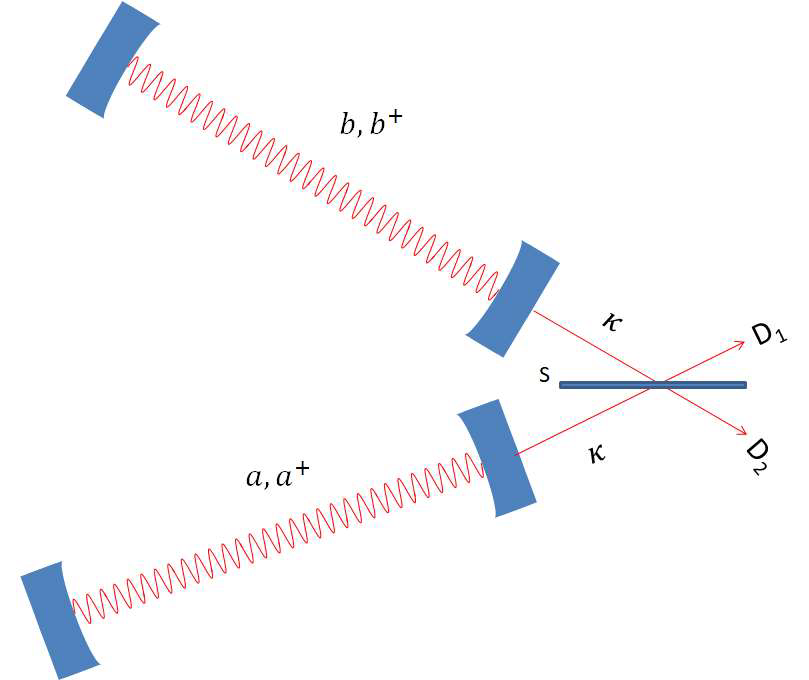
\includegraphics[width=0.5\textwidth]{fig2.png}
    \caption{Output of two cavities are mixed by splitter $S$ and detected by photon-counter $D_1$ and $D_2$}
    \label{fig:prob-2}
\end{figure}

\paragraph{Stochastic wavefunction of two cavity fields} We consider the setup in \prettyref{fig:prob-2}, the leak fields of two identical cavities are mixed by a beamsplitter $S$ and then detected by the photon counter D1 and D2. Following the stochastic wavefunction method, the effective Hamiltonian for the photon field of the twocavity system can be written as $H_{\text {eff }}=\hbar\left(-i \frac{\kappa}{2}\right)\left(a^{+} a+b^{+} b\right)$. While normally we would have quantum jump operators of $C_{a}=\sqrt{\kappa} a$ and $C_{b}=\sqrt{\kappa} b$, here it is more convenient to introduce collective jump operators $C_{1}=\sqrt{\kappa}(t a+r b)$ and $C_{2}=\sqrt{\kappa}\left(-r^{*} a+t b\right)$, with $r, t$ to be the reflective and transmission coefficients of the beamsplitter $S$.

\begin{itemize}
    \item[2.1] Consider the initial state to be a product coherent state: $|\psi(0)\rangle=|\alpha, \beta\rangle$.
    Evaluate the stochastic wavefunction of the photon field, $\left|\psi_{\mathrm{S}}(\mathrm{t})\right\rangle$, for the non-Hermitian evolution without any quantum jump, and after a quantum jump by $C_{1}$ operator (D1 "click")
    \item[2.2] Consider the simple situation of a $50 \%$ beamspitter, $r=t=1 / \sqrt{2}$, continue with the first problem to derive the photon detection rate $\gamma_{1}(t)=\left\langle\psi(t)\left|C_{1}^{+} C_{1}\right| \psi(t)\right\rangle$ and $\gamma_{2}(t)=\left\langle\psi(t)\left|C_{2}^{+} C_{2}\right| \psi(t)\right\rangle$. Is it possible to properly choose non-zero $\alpha$ and $\beta$ values, so as to have $\gamma_{1} \equiv 0$ ?
    \item[2.3] Repeat $2.1$ with the Fock initial state $|\psi(0)\rangle=|N, N\rangle$.
    \item[2.4] Continue with 2.2, again assuming $r=t=1 / \sqrt{2}$, evaluate $\gamma_{1}(t)=\left\langle\psi(t)\left|C_{1}^{+} C_{1}\right| \psi(t)\right\rangle$ and $\gamma_{2}(t)=\left\langle\psi(t)\left|C_{2}^{+} C_{2}\right| \psi(t)\right\rangle$ before there is any quantum jump, and after a quantum jump with a $D_{1}$ "click". For $N=1$. Discuss your results in terms of the HongOu-Mandel effect.
\end{itemize}

\paragraph{Solution}

\paragraph{}

\paragraph{Cavity QED and single photon source} As in the figure above, consider a 2-level atom coupled to a cavity field with single-photon Rabi frequency $g_{a c}$. The atom is in addition subjected to a laser field excitation from the side with a Rabi frequency $\Omega(\mathrm{t})$. Taking into account the radiative decay by the atom and the leak of the cavity, the effective Hamiltonian of the controlled and coupled system is given by
\begin{equation}
    H_\text{eff}=\hbar\left(- \ii \frac{\Gamma}{2}\right)|e\rangle\langle e|+\hbar\left(-\Delta- \ii \frac{\kappa}{2}\right) a^{+} a+\left[\hbar\left(\frac{\Omega(\mathrm{t})}{2}+g_{a c} a\right)|e\rangle\langle g|+\text { h.c. }\right],
\end{equation}
where $\Delta=\omega-\omega_{e g}$ is the detuning of the cavity mode frequency from the atomic resonant frequency. The collapse operators are given by $C_{1}=\sqrt{\Gamma}|g\rangle\langle e|$ and $C_{2}=\sqrt{\kappa} a$.
3a) Consider $\Omega(\mathrm{t})=0$ and with system initially in $\left|\psi_{S}(0)\right\rangle=|g, n=1\rangle$, that is, the atom is in the ground state and the cavity mode is in $\mathrm{n}=1$ Fock state. Consider good cavity $(\kappa \ll g, \Gamma)$ and weak coupling $(g \ll \Delta, \Gamma)$ limits. Expand $\left|\psi_{S}(t)\right\rangle$ in proper basis of choice, and to derive the Schrodinger equation for the coefficients of the stochastic wavefunction, without quantum jump. Perturbatively derive the system decay rate $ \gamma_{1}(t)=\left\langle\psi_{S}\left|C_{1}^{+} C_{1}\right| \psi_{S}\right\rangle$ and $ \gamma_{2}(t)=\left\langle\psi_{S}\left|C_{2}^{+} C_{2}\right| \psi_{S}\right\rangle$ (i.e., using the adiabatic elimination method which assumes $\left|\psi_{S}(t)\right\rangle \approx\left|\widetilde{\psi}_{S}\right\rangle$, with $\left.H_\text{eff}\left|\widetilde{\psi_{S}}\right\rangle \approx-\Delta-\frac{i \kappa}{2}\left|\widetilde{\psi_{S}}\right\rangle\right)$.
3b) Repeat Question 3a, but with system initially in $|\psi\rangle=|e, n=0\rangle$ and in the bad cavity $(\kappa\rangle\rangle$ $g, \Gamma)$ and weak coupling $(g \ll \Delta, \Gamma)$ limit. You should arrive at a total decay rate $\gamma=\gamma_{1}+\gamma_{2}$ that describes the Purcell effect as in the class. Discuss the condition under which $\gamma_{2} \gg \gamma_{1}$, that is, the decay of the system more likely leading to a single photon emission into the cavity leak mode.
3c) With the system initially in $|\psi\rangle=|g, n=0\rangle$ and with a resonant pulse $\Omega(t)=$ $\Omega_{0} \sin \left(\frac{\pi t}{\tau}\right)$ switched on and off smoothly for $0<t<\tau$. Assuming $|\psi(t)\rangle$ to be driven by the 2-level Hamiltonian $H_{a}=H_{e f f}(t ; \Gamma, \kappa, g \rightarrow 0) \quad$ [note: this happens effectively when $\Gamma, \kappa, g \ll$ $1 / \tau]$. Now, putting back all the parameters into $H_\text{eff}$, Calculate $\gamma_{1}(t)=\left\langle\psi\left|C_{1}^{\dagger} C_{1}\right| \psi\right\rangle$ and $\gamma_{2}(t)=\left\langle\psi\left|C_{2}^{\dagger} C_{2}\right| \psi\right\rangle$ for stochastic wavefunction without quantum jump during $0<\mathrm{t}<\mathrm{T}$, with $T \gg \frac{1}{\kappa}, \frac{1}{\Gamma}$
4d) Discuss $\Omega(t)$ and other parameters in Eq. (2), so that a single photon can be deterministically generated into the cavity leaking mode with high efficiency. Discuss the form of the single-photon wavefunction, and the fidelity of the single-photon source (how likely there is exactly one photon in the time-dependent leaky mode).

\paragraph{Solution}

\end{document}